% AAAI 2027 ABER Supplementary Material (standalone, separate PDF)
\documentclass[letterpaper]{article}
\usepackage[submission]{aaai2027}
\usepackage[hyphens]{url}
\usepackage{graphicx}
\urlstyle{rm}
\def\UrlFont{\rm}
\usepackage{amsmath,amssymb,amsfonts}
\usepackage{booktabs}
\usepackage{multirow}
\usepackage{caption}
\frenchspacing

\pdfinfo{/TemplateVersion (2027.1)}
\setcounter{secnumdepth}{0}
\title{ABER: Supplementary Material}
\author{Anonymous Submission}
\affiliations{}

\begin{document}
\maketitle

\section{Scope and Method Identity}

This supplement concerns only ABER, the forward/turn sampled-data filter
defined in the main paper.  Its deployed action is the normalized pair
$(u^f,u^\omega)$; it does not assume a Cartesian acceleration command.
The implementation entry point is
\path{safe_rl/filters/aber.py}, which exports \texttt{ABERFilter} from
\path{safe_rl/filters/brake_manifold.py}.  The latter filename and the
\texttt{BrakeManifoldFilter} alias are retained only so historical
configuration files and checkpoints remain loadable.

Earlier diagnostic material in the repository studied other safety-filter
designs.  Their propositions and experiments are not used as evidence for the
current paper.  The current empirical claims are backed by eight checked-in
evidence groups:
\begin{enumerate}
\item \path{data/aber_property_tests.json}, the seeded falsification audit;
\item \path{data/certified_diffdrive_benchmark.json}, generated by the
fixed theorem-envelope benchmark;
\item \path{data/aber_component_ablation.json} and its raw JSONL.GZ,
covering 295,200 component-study records;
\item \path{data/safetygym_aber_matrix.json} and the exactly reproduced
\path{data/safetygym_aber_matrix_retrained.json}, audited aggregates of 30
training cells and 1,500 deterministic evaluation episodes;
\item \path{data/aber_runtime_scaling.json} and its raw JSONL.GZ, covering
one million timed projection calls;
\item \path{data/aber_paired_matrix.json}, the strict-ABER paired audit and
its independent verification report;
\item \path{data/aber_safetygym_contract_v1.json} plus 30 raw trace files,
the frozen 600-episode A1--A2 substep audit reported in
Section~\ref{sec:sg-contract-v1}; and
\item \path{full_30_checkpoint_aggregate.json} and
\path{cross_task_audit.json}, the complete filter-off/strict/ABER-LR
30-checkpoint analysis.
\end{enumerate}
The paired evidence additionally hashes all 30 exact policy checkpoints,
resolved training configurations, raw episode and step files, and generating
scripts.  These checkpoints are not used by any theorem or component-study
claim.

\section{Acceptance Envelope and Recovery}

For obstacle $i$, let
$d_i(q)=\|q-o_i\|-r_i$ and
$D(s)=s^2/(2a_b)$.  ABER certifies the intersection
\[
 \mathcal C=\{(q,s):d_i(q)-D(s)\ge0\ \text{for every }i\}.
\]
The normal branch uses the measurable envelope
\[
 s^+\le\max\{s,v_{\max}|u^f|\},\qquad
 \ell\le\Delta t\max\{s,v_{\max}|u^f|\}.
\]
Writing $z$ for the common upper bound, the sufficient one-step condition is
\[
 \Delta t z+D(z)\le d_{\min},\qquad
 d_{\min}=\min_i d_i(q).
\]
Its nonnegative inverse is
\[
 z_{\max}=\min\!\left\{v_{\max},
 -a_b\Delta t+
 \sqrt{(a_b\Delta t)^2+2a_bd_{\min}}\right\}.
\]
If $s\le z_{\max}$, the implementation clips only $u^f$ to
$[-z_{\max}/v_{\max},z_{\max}/v_{\max}]$ and retains the requested turn.
Otherwise it sends the executable recovery $(0,0)$.

\subsection{Cap maximality and its boundary}

For $d\ge0$, define
$g(z)=\Delta t z+z^2/(2a_b)$.  Since
$g'(z)=\Delta t+z/a_b>0$ for $z\ge0$, $g$ is strictly increasing and the
unclipped expression above is its unique nonnegative inverse.  Consequently,
\[
 z_{\max}(d)=\max\{z\in[0,v_{\max}]:g(z)\le d\}.
\]
When $z_{\max}<v_{\max}$, every larger speed violates the robust one-step
condition.  This is a sharpness statement only within ABER's
direction-independent A1 envelope: a controller using obstacle bearing or
turn geometry may certify a larger action in a particular state.

\subsection{Semi-implicit recovery check}

The main theorem accepts any measured recovery envelope satisfying
\[
 \ell^{\rm rec}+D(s^+)\le D(s).                 \tag{S1}
\]
For the benchmark plant,
\[
 s^+=\max\{s-a_b\Delta t,0\},\qquad
 \ell^{\rm rec}\le\Delta t s^+.
\]
When $s<a_b\Delta t$, both $s^+$ and the upper bound on path length are zero.
Otherwise,
\begin{align*}
 \ell^{\rm rec}+D(s^+)
 &\le \Delta t(s-a_b\Delta t)
   +\frac{(s-a_b\Delta t)^2}{2a_b}\\
 &=\frac{s^2}{2a_b}-\frac12a_b\Delta t^2
 \le D(s),
\end{align*}
which proves (S1).  This derivation is specific to the accepted low-level
envelope; it is not inferred merely from the commanded setpoint.

\subsection{Why one recovery covers multiple obstacles}

Distance to each static obstacle is 1-Lipschitz with respect to path length:
$d_i(q^+)\ge d_i(q)-\ell$.  Therefore, in the normal branch,
\[
 d_i(q^+)-D(s^+)
 \ge d_{\min}-\Delta t z_{\max}-D(z_{\max})\ge0
\]
for every $i$.  In recovery, (S1) gives
\[
 d_i(q^+)-D(s^+)\ge d_i(q)-D(s)\ge0
\]
for every $i$ simultaneously.  No intersection of obstacle-dependent
directional half-spaces is required.  Heterogeneous physical radii are
supported by
\texttt{reset(obstacles, obstacle\_radii=...)}; callers that omit the
optional list retain the configured common hazard radius.  Position
uncertainty is added to every keepout radius before clearances are computed.

\section{Code-to-Paper Mapping}

\begin{table}[t]
\centering
\small
\setlength{\tabcolsep}{4pt}
\begin{tabular}{p{0.24\linewidth}p{0.32\linewidth}p{0.34\linewidth}}
\toprule
Paper object & Implementation & Test or data evidence\\
\midrule
$d_{\min}$ and $D(s)$ &
\path{ABERFilter.project} &
heterogeneous-radius and uncertainty tests\\
$z_{\max}$ inverse &
\path{ABERFilter.speed_cap} &
5000 inversion/sharpness checks\\
$(0,0)$ recovery &
\path{project}; \path{recovery_speed_bound} &
executable-recovery and adversarial-start tests\\
forward/turn action map &
\texttt{project} &
Cartesian action rejection; turn retention\\
component necessity &
\path{experiments/aaai/aber_component_ablation.py} &
295,200 raw boundary/navigation records\\
certified benchmark &
\path{experiments/aaai/certified_diffdrive_benchmark.py} &
200 episodes per method across two scene families\\
Safety-Gym aggregation &
\path{experiments/aaai/aggregate_aber_matrix.py} &
30 manifests, saved Hydra configs, 1500 evaluations\\
runtime scaling &
\path{experiments/aaai/aber_runtime_scaling.py} &
1,000,000 real \texttt{project} timings\\
paired policy matrix &
\path{run_aber_latched_restore_cross_task_multiseed.py};
\path{audit_aber_latched_restore_cross_task_multiseed.py} &
30 checkpoints, 15,000 filtered paired rollouts\\
\bottomrule
\end{tabular}
\caption{Direct mapping from the current ABER paper to code and evidence.}
\label{tab:mapping}
\end{table}

The public filter rejects \texttt{action\_form=cartesian}.  Historical safety
identifiers \texttt{brake\_manifold} and \texttt{saber} dispatch to the same
\texttt{ABERFilter}; they do not select separate algorithms.  The focused
test command is:
\begin{quote}
\noindent\path{PYTHONPATH=.}\ \path{pytest}\ \path{-q}\ \path{tests/test_brake_manifold_sampled_data.py}\par
\noindent\path{PYTHONPATH=.}\ \path{pytest}\ \path{-q}\ \path{tests/test_aber_component_ablation.py}
\end{quote}
The complete focused filter suite reports 25 passed tests in the archived
environment.

\section{Falsifiable Property Audit}

The seeded script
\path{experiments/aaai/certify_aber_properties.py} records source hashes,
parameters, environment versions, and up to 20 counterexamples per failed
property before exiting nonzero.  It checks 5000 analytic cap inversions and
26,354 normal/recovery projections over one, two, and eight heterogeneous
static obstacles.  The latter count includes every normal sample plus every
sample for which a certified recovery state exists.  No required property
fails.

The same script deliberately violates the calibration premise by setting
actual braking to $0.5a_b$ while retaining the accepted envelope in the
certificate.  All 5000 samples then produce a negative next-step barrier.
These expected counterexamples demonstrate that $(0,0)$ is a certified
recovery only after A2 has been established for the deployed low-level
controller.

\section{Component Necessity and Calibration Study}

The component study crosses four control periods
$\{0.02,0.05,0.10,0.20\}$~s, four actual/configured braking ratios
$\{0.5,0.75,1.0,1.25\}$, and $m\in\{1,4,8\}$ obstacles.  Its three
variants are full ABER, ABER without the sampled displacement $\Delta t z$,
and ABER without the distinct $(0,0)$ recovery branch.  Each grid cell has
1,000 samples for each boundary challenge and 50 navigation episodes.

\subsection{Boundary controls}

The sampled-term challenge initializes $d=\Delta t s+D(s)$; the recovery
challenge initializes $d=D(s)$.  The former makes the full normal inequality
tight, while the latter requires the A2 witness.  Table~\ref{tab:boundary}
pools equal-size calibrated or under-braking cells only after all 48
predeclared per-grid checks pass.

\begin{table}[t]
\centering
\small
\setlength{\tabcolsep}{3.2pt}
\begin{tabular}{llrr}
\toprule
Calibration & Variant/challenge & Trials & Viol.\\
\midrule
$\rho\ge1$ & Full / sampled term & 24,000 & 0\\
$\rho\ge1$ & Full / recovery & 24,000 & 0\\
$\rho\ge1$ & No sampled term / sampled term & 24,000 & 24,000\\
$\rho\ge1$ & No recovery / recovery & 24,000 & 24,000\\
$\rho<1$ & Full / recovery & 24,000 & 24,000\\
\bottomrule
\end{tabular}
\caption{Predeclared one-step controls.  Violation means a negative
next-state braking-envelope certificate; no row is selected post hoc.}
\label{tab:boundary}
\end{table}

One-step certificate violation is deliberately the primary endpoint.  A
sample can leave the recursively certified set before it crosses the obstacle
surface, so zero immediate collisions would not rescue a failed certificate.

\subsection{Navigation results}

Among calibrated episodes, full ABER has 0/1,200 violation episodes and
0/1,200 collisions, with 1,186 successes and 14 horizon timeouts.  Removing
the sampled term yields 1,200/1,200 violation episodes, 481 collisions, and
719 successes.  Removing recovery yields 1,002 violation episodes, 298
collisions, and 902 successes.  Under braking ratios below one, full ABER
itself produces 873/1,200 violation episodes and 539 collisions, which is the
intended negative control for a false A2 calibration.

The artifact stores 288,000 individual boundary records and 7,200 navigation
records as deterministic gzip JSON Lines.  Two complete runs produced the
same raw SHA-256, recorded in the manifest.  The aggregate also records hashes
of the exact filter and generation script.

\section{Certified-Envelope Benchmark Details}

The benchmark uses
$\Delta t=0.1$~s, $v_{\max}=1$~m/s,
$a_{\rm acc}=a_b=0.9$~m/s$^2$,
$|\omega|\le1.5$~rad/s, and $r_i=0.25$~m.
The state update is semi-implicit: the bounded velocity servo is applied
first, then the next speed is held over the position update.  All methods use
the same reactive navigator and the same 100 fixed seeds in each scene.
The three comparison filters are fixed geometry-specialized reference
implementations, not claimed reproductions of every tuning choice in their
source papers.

\begin{table}[t]
\centering
\small
\setlength{\tabcolsep}{2.4pt}
\begin{tabular}{llrrrrrr}
\toprule
Scene & Method & Coll. & Succ. & Time & min clr. & Path & Interv.\\
 & & (\%) & (\%) & (s) & worst (m) & (m) & mean\\
\midrule
\multirow{4}{*}{Single}
& Braking CBF & 0 & 100 & 5.80 & 0.290 & 4.30 & 40.85\\
& SD-CBF/ZOCBF & 0 & 100 & 4.90 & 0.185 & 4.30 & 33.77\\
& Collision cone & 0 & 100 & 5.91 & 0.083 & 4.41 & 59.10\\
& ABER & 0 & 100 & 6.46 & 0.016 & 4.22 & 32.26\\
\midrule
\multirow{4}{*}{Multi}
& Braking CBF & 0 & 100 & 7.22 & 0.220 & 4.85 & 70.00\\
& SD-CBF/ZOCBF & 0 & 100 & 5.55 & 0.046 & 4.86 & 55.39\\
& Collision cone & 0 & 100 & 7.33 & 0.001 & 5.06 & 73.28\\
& ABER & 0 & 100 & 7.22 & 0.016 & 4.80 & 60.40\\
\bottomrule
\end{tabular}
\caption{Full fixed-envelope aggregate.  Each cell has 100 episodes.}
\label{tab:certfull}
\end{table}

ABER invokes recovery 866 times in the single-obstacle set and 1335 times in
the multi-obstacle set, with zero recorded certificate violations.  All four
methods have zero collisions and 100\% goal success.  Accordingly, this
experiment supports implementation consistency and task completion inside
the accepted envelope; it does not support an unsafe-baseline claim.

\section{Safety-Gymnasium Audit}

The matrix crosses three tasks, two reward modes, and five training seeds.
Each run uses 200K environment steps and 50 deterministic evaluation episodes.
All 30 cells disable EKF/IMU estimation and action-correction calibration.
The saved Hydra configurations are checked for a normalized forward/turn
action, $a_b=0.9$, $\Delta t=0.02$, $v_{\max}=1.5$, a 0.05~m safety margin,
and task-specific hazard radius.  The aggregation script aborts on a missing
run, missing metric, unexpected configuration value, or an evaluation count
other than 50.

\begin{table*}[t]
\centering
\small
\setlength{\tabcolsep}{4.0pt}
\begin{tabular}{llrrrrr}
\toprule
Mode & Task & Cost & Reward & Succ. (\%) & worst clr. & deep steps\\
\midrule
Native & Goal1 & $79.24\pm93.52$ & $-6.97\pm9.78$ & $39.2\pm18.1$ & -0.075 & 26.30\\
Native & Push1 & $5.85\pm7.91$ & $0.28\pm0.14$ & $1.6\pm1.7$ & -0.497 & 58.29\\
Native & Goal2 & $26.73\pm40.55$ & $-1.33\pm3.79$ & $21.6\pm11.3$ & -0.039 & 0.00\\
\midrule
+sim-BRT & Goal1 & $16.86\pm20.35$ & $-1.53\pm2.22$ & $24.8\pm17.8$ & -0.017 & 0.00\\
+sim-BRT & Push1 & $36.48\pm52.32$ & $0.23\pm0.05$ & $0.8\pm1.8$ & -0.468 & 42.03\\
+sim-BRT & Goal2 & $21.44\pm14.40$ & $-0.70\pm0.82$ & $12.0\pm11.3$ & -0.009 & 0.00\\
\bottomrule
\end{tabular}
\caption{Audited ABER matrix.  Mean$\pm$sample standard deviation is across
five seeds.  Worst clearance is over 250 evaluation episodes per cell; deep
steps use the pre-declared $-0.05$~m threshold.}
\label{tab:sgfull}
\end{table*}

These results are empirical and are not presented as validation of the global
A1--A2 servo envelope.  sim-BRT reduces cost on Goal1 and Goal2, increases it
on Push1, and lowers mean goal success in all three tasks.  Push clearance
includes box--hazard geometry, which lies outside the robot--obstacle
certificate.  The paper therefore reports native and shaped training
separately and makes no claim that reward shaping is uniformly beneficial.

\section{Runtime Scaling Audit}

The runtime experiment invokes the submitted \texttt{ABERFilter.project}
implementation directly.  It crosses
$m\in\{0,1,2,4,8,16,32,64,128,256\}$, with 20 repeats and 5,000 calls per
repeat, for exactly one million retained timing records.  Positions,
velocities, and actions are generated before timing; only \texttt{project} is
inside \texttt{perf\_counter\_ns}.  Serialization, policy inference, and
environment stepping are excluded.  Count order is reversed on alternating
repeats, each cell receives 200 warm-up calls, and the process is pinned to one
core of an Intel i7-13850HX.

\begin{table}[t]
\centering
\small
\setlength{\tabcolsep}{5pt}
\begin{tabular}{rrrr}
\toprule
$m$ & Median ($\mu$s) & p95 ($\mu$s) & p95/20 ms (\%)\\
\midrule
0 & 6.14 & 6.46 & 0.032\\
1 & 17.96 & 18.82 & 0.094\\
8 & 19.35 & 21.57 & 0.108\\
32 & 27.80 & 30.80 & 0.154\\
128 & 57.35 & 61.79 & 0.309\\
256 & 98.53 & 103.76 & 0.519\\
\bottomrule
\end{tabular}
\caption{Observed wall time over 100,000 calls per listed count except that
all ten counts, including omitted intermediate rows, are present in raw data.}
\label{tab:runtimesupp}
\end{table}

For positive counts, least-squares fitting of the pooled per-count median gives
$0.3168m+17.1084$~$\mu$s with $R^2=0.99961$.  This is empirical scaling on
one machine, not the complexity proof; the $O(m)$ result follows independently
because the implementation performs one vectorized distance reduction and a
constant amount of scalar work.  Exact source and raw-data hashes are recorded
in the aggregate and checksum manifest.

\section{Paired Learned-Policy Safety--Liveness Audit}

We retrain 30 policies: native and sim-BRT training on Goal1, Push1, and Goal2,
with five training seeds per cell and 200K environment steps per policy.  Each
atomic checkpoint contains the actor tensors, resolved configuration, training
metadata, and SHA-256 digest.  The resulting training-matrix aggregate exactly
reproduces all 192 scalar statistics in the earlier audited aggregate
(maximum absolute difference zero).

Each checkpoint is evaluated with deterministic policy actions under three
execution conditions: filter off, strict ABER, and the frozen ABER-LR
extension.  Each filtered variant is paired with filter-off execution through
the same checkpoint, reset seed, and canonical initial snapshot, including
robot, goals, obstacles, walls, and the Push box.  Native Goal1 uses reset
seeds 44000--44249; the remaining 25 checkpoints use 45000--45249.  The two
filter-off reruns are identical at the decoded-record level.  All checkpoint
and initial-state hashes match.  No seed is searched, discarded, selectively
rerun, or imputed.

ABER-LR uses
\[
(\epsilon,a_b,s_{\rm stop},u^f_{\rm restore},k_\omega)
=(0.10,0.9,0.05,0.25,1.0).
\]
Directional restore is enabled and latched; the separate escape heuristic is
disabled.  These values were frozen before the five remaining mode--task
groups were evaluated.  Goal1 was the development group used to choose the
candidate; the cross-task matrix is therefore the transfer test.  We report
all groups rather than selecting only those that pass the development gate.

For each condition, the primary joint endpoint is
\[
\mathrm{SCR}=\Pr(\mathrm{success}\land
                  \neg\mathrm{geometric\ collision}).
\]
Collision is negative physical surface clearance; Push uses the minimum of
robot--hazard and box--hazard clearance.  SCR is always accompanied by raw
success, collision, unsafe success, and timeout, so it does not conceal the
marginal tradeoff or introduce a tuned scalarization weight.
Each checkpoint contributes one 250-episode rate difference.  Reported 95\%
intervals are percentile intervals from 50,000 seeded bootstrap resamples of
the 30 checkpoint differences; episodes are never treated as independent
training replicates.  Equal-group and equal-checkpoint weighting coincide
because every mode--task group contains five checkpoints.

\subsection{Failure Definition and Rejected Repairs}

A negative test is not automatically a collision failure.  We distinguish:
(i)~\emph{safety failure}, crossing the frozen collision bound;
(ii)~\emph{liveness failure}, missing the success or recovery-tail target;
(iii)~\emph{coordination failure}, missing the joint SCR target despite an
improved marginal; and (iv)~\emph{transfer failure}, losing the required
direction or magnitude across training seeds or tasks.  A separate
\emph{contract failure} means that A1--A2 cannot be attached to the empirical
plant; it does not erase an empirical collision result.

The 250-pair yaw-escape pilot required at least +10 success points with no
more than +3 collision points.  The later cross-task gate requires at least
+10 success points, no collision increase, at least +5 SCR points, and SCR
improvement in at least four of five training seeds.  The 50-pair margin
screen was discovery-only: it selected a candidate but could not pass the
method by itself.  Table~\ref{tab:rejected-repairs} retains the negative
results that determined the final mechanism.

\begin{figure*}[t]
  \centering
  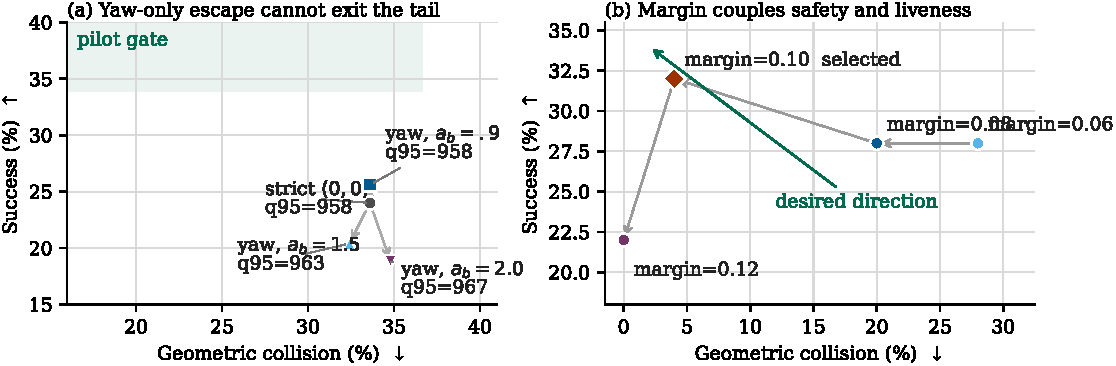
\includegraphics[width=0.98\textwidth]{../figures/supplement/aber_lr_failure_landscape.pdf}
  \caption{Failure landscape on the Goal1 development checkpoint; upper-left
  is favorable.  (a)~Each yaw-only point uses 250 matched episodes.  The
  shaded gate requires success $\ge34\%$ and collision $\le36.6\%$; q95
  recovery streaks remain near the 1000-step horizon.  (b)~A separate
  50-pair discovery screen exposes the margin tradeoff.  Margin 0.10 was
  selected for disjoint confirmation; arrows connect settings only to show
  the frozen search order, not a continuous interpolation.}
  \label{fig:aber-lr-failure-landscape}
\end{figure*}

\begin{table*}[t]
\centering
\small
\setlength{\tabcolsep}{3.0pt}
\begin{tabular}{p{0.19\textwidth}rrrrrp{0.31\textwidth}}
\toprule
Attempt (Goal1, one checkpoint) & Pairs & Succ. & Coll. & Rec. & q95 & Decision and diagnosed difficulty\\
 & & \multicolumn{4}{c}{\% except q95 steps} & \\
\midrule
Strict $(0,0)$ recovery & 250 & 24.0 & 33.6 & 72.0 & 958 & Liveness failure: the recovery tail occupies nearly the horizon.\\
Yaw-only escape, $a_b=0.9$ & 250 & 25.6 & 33.6 & 70.7 & 958 & Fail: only +1.6 success points; turning does not change position or clearance.\\
Yaw-only escape, $a_b=1.5$ & 250 & 20.4 & 32.4 & 68.8 & 963 & Fail: fewer recovery entries, but the tail persists and success falls.\\
Yaw-only escape, $a_b=2.0$ & 250 & 18.8 & 34.8 & 68.2 & 967 & Fail: success and collision both move unfavorably relative to $a_b=0.9$.\\
Latched restore, margin 0.06 & 50 & 28.0 & 28.0 & -- & -- & Discovery-only safety problem: intervention remains too late.\\
Latched restore, margin 0.10 & 50 & 32.0 & 4.0 & -- & -- & Selected balance; sent to fresh-seed confirmation.\\
Latched restore, margin 0.12 & 50 & 22.0 & 0.0 & -- & -- & Coordination risk: eliminating collision alone restores conservatism.\\
Margin-0.10 held-out confirm & 250 & 32.8 & 7.6 & 26.8 & 130 & Single-checkpoint pass; still insufficient for cross-task generalization.\\
\bottomrule
\end{tabular}
\caption{Rejected-repair audit and the held-out transition to ABER-LR.
Success, collision, and recovery occupancy are filter-on rates.  Rows use
their stated, disjoint discovery/pilot/confirmation schedules and must not be
pooled.  q95 is the episode-level maximum recovery-streak percentile.}
\label{tab:rejected-repairs}
\end{table*}

The structural difficulty is therefore two-sided.  With zero translational
authority, recovery cannot increase clearance; changing $a_b$ changes when
recovery is entered but not how it exits.  Once translation is introduced,
the margin must be large enough to absorb its empirical risk but not so large
that early intervention recreates the original liveness loss.  Latching is
needed for persistence until certificate re-entry.  These coupled choices
explain why a single collision or success number is not an adequate test.

\begin{table*}[t]
\centering
\small
\setlength{\tabcolsep}{3.1pt}
\begin{tabular}{llrrrrrrc}
\toprule
Training & Task & Off SCR & Strict SCR & LR SCR &
$\Delta_{\rm LR-strict}$ SCR & $\Delta_{\rm LR-strict}$ Coll. &
$\Delta_{\rm LR-off}$ SCR & Gate\\
 & & \multicolumn{6}{c}{percentage points} & \\
\midrule
Native & Goal1 & 47.52 & 37.68 & 56.64 & +18.96 & -8.80 & +9.12 & pass\\
Native & Push1 & 4.16 & 3.36 & 4.08 & +0.72 & +0.48 & -0.08 & fail\\
Native & Goal2 & 39.60 & 27.60 & 46.08 & +18.48 & -2.80 & +6.48 & pass\\
sim-BRT & Goal1 & 37.68 & 32.64 & 43.20 & +10.56 & -0.72 & +5.52 & pass\\
sim-BRT & Push1 & 2.48 & 2.16 & 3.44 & +1.28 & -4.08 & +0.96 & fail\\
sim-BRT & Goal2 & 24.32 & 15.84 & 23.84 & +8.00 & -1.44 & -0.48 & fail\\
\bottomrule
\end{tabular}
\caption{Complete group-level paired analysis.  Negative collision difference
is favorable.  The strong gate requires at least +10 success points, no
collision increase, at least +5 SCR points, and SCR improvement in at least
four of five training seeds.}
\label{tab:aber-lr-groups}
\end{table*}

\paragraph{Strict ABER versus filter off.}
Equal-weight checkpoint means show the intended safety effect and the
liveness failure: collision falls from 43.19\% to 7.11\%, while success falls
from 42.48\% to 19.92\% and timeout rises from 57.52\% to 80.08\%.  SCR falls
from 25.96\% to 19.88\%.  Thus collision reduction alone is not an adequate
summary of a safety filter attached to a goal-directed policy.

\paragraph{ABER-LR versus strict ABER.}
ABER-LR raises success by 9.79 points (checkpoint bootstrap 95\% CI
$[6.49,13.37]$), lowers collision by 2.89 points
($[1.11,5.13]$ reduction), raises SCR by 9.67 points
($[6.37,13.33]$), and lowers timeout by 9.79 points
($[6.47,13.40]$ reduction).  All six group means and 28/30 checkpoint cells
improve SCR.  The strong development-sized gate passes in three groups:
Native Goal1, Native Goal2, and sim-BRT Goal1.  Native Push1 is the only group
with a collision increase (+0.48 points), and its unfiltered success is only
5.12\%, limiting the available completion signal.

The three gate failures have different meanings.  Native Push1 is a safety
and coordination miss (+0.48 collision and only +0.72 SCR points).
sim-BRT Push1 moves collision and SCR in the favorable direction but cannot
reach the magnitude gate because its unfiltered success is only 4.64\%.
sim-BRT Goal2 improves SCR in all 5/5 checkpoints but its +8.00-point mean
misses the +10 success threshold.  The latter two are magnitude/transfer
limitations, not reversals of the recovery mechanism.

\paragraph{ABER-LR versus filter off.}
Collision falls by 38.97 points and unsafe success by 16.36 points.  Mean SCR
rises by 3.59 points (95\% CI $[1.03,6.37]$), although raw success falls by
12.77 points and timeout rises by 12.77 points.  This SCR improvement is
positive in four of six group means and 17/30 checkpoint cells (nonnegative
in 19/30), not universal.  The supported claim is therefore improved
coordination on average, and consistent improvement relative to strict ABER,
not dominance of the unfiltered policy.

\begin{figure}[t]
  \centering
  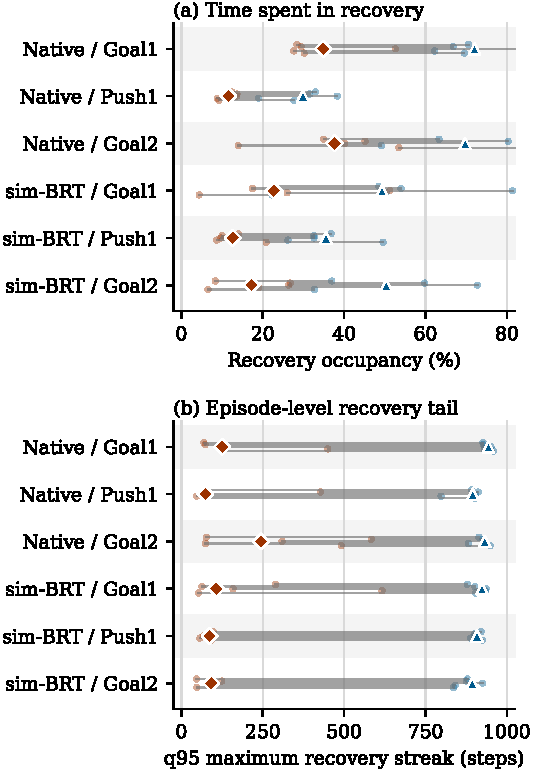
\includegraphics[width=\columnwidth]{../figures/supplement/aber_lr_recovery_mechanism.pdf}
  \caption{Recovery mechanism by mode--task group.  Small points show the
  five checkpoints; large blue triangles and orange diamonds show strict
  ABER and ABER-LR group means, with matched checkpoints linked in gray.
  Mean occupancy falls from 51.15\% to 22.76\%, and group-average q95 maximum
  streak from 916 to 121 steps.}
  \label{fig:aber-lr-recovery-supp}
\end{figure}

The full-matrix pattern in Fig.~\ref{fig:aber-lr-recovery-supp} supports the
proposed mechanism: strict $(0,0)$ recovery creates long episodes of immobility
that terminate at the horizon, whereas latched directional restore shortens
the recovery tail.  Timeout falls by the same 9.79 points by which success
rises.  This is empirical liveness evidence, not a certificate for restore.
Push includes movable-box dynamics outside the robot/static-obstacle theorem,
so neither Push result is used as theorem validation.

\section{Intervention Event Audit}

\renewcommand{\thefigure}{S\arabic{figure}}
\setcounter{figure}{0}

This separate, earlier strict-ABER audit diagnoses the failure mode that
motivated ABER-LR; it is not used to estimate the three-arm effect sizes in
Table~\ref{tab:aber-lr-groups}.  We reconstruct events directly from the
11,860,270 paired step records and
use only the 6,485,664 filter-on steps.  An intervention event, recovery
event, or uncertified run is a maximal contiguous run of the corresponding
Boolean indicator within one episode.  Runs never cross episode boundaries.
The six training-mode/task cells retain their original 1,250 filter-on
episodes each; no episode, action, or threshold is added by this audit.

\begin{figure*}[t]
\centering
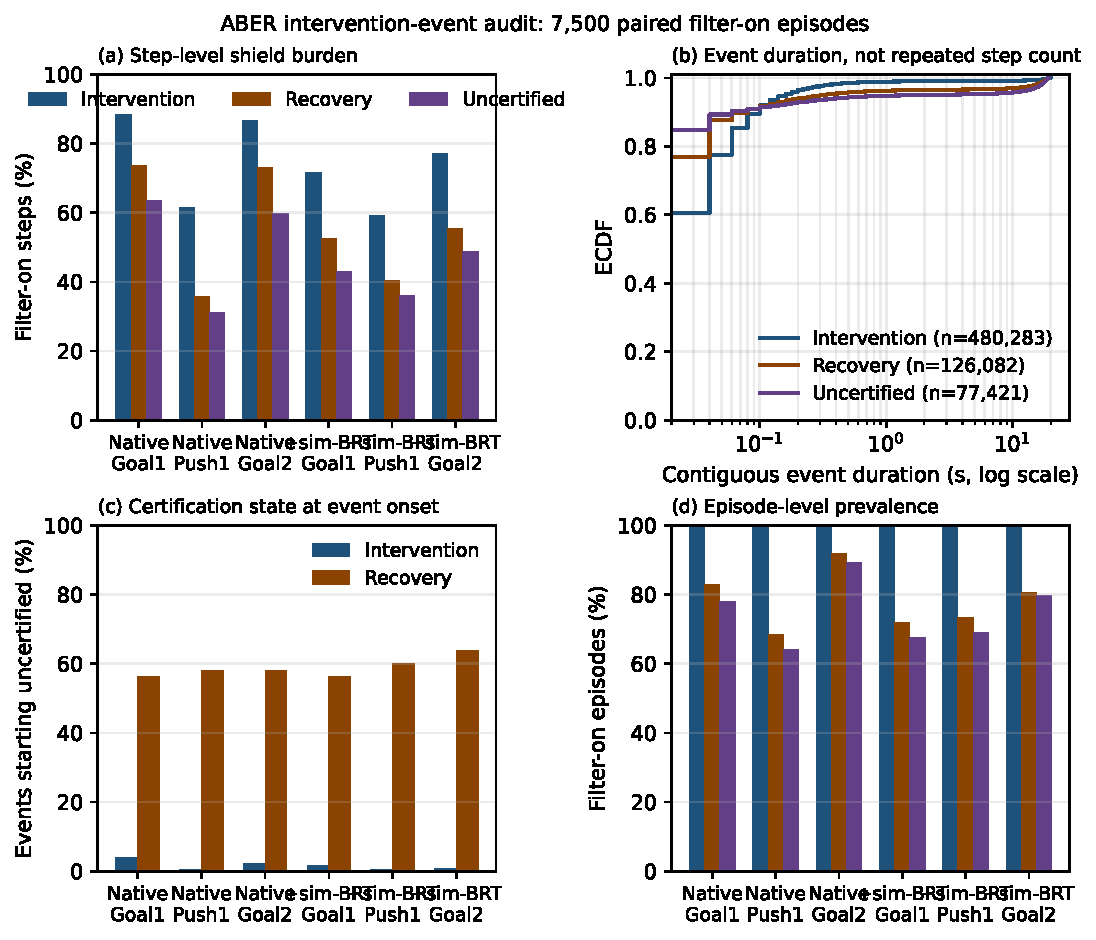
\includegraphics[width=\textwidth]{../figures/supplement/aber_intervention_event_audit.pdf}
\caption{Event-level reconstruction over all 7,500 filter-on episodes.
An event is a maximal contiguous run within one episode. Most interventions
are one-step corrections, but a small tail of long recovery/uncertified runs
dominates time under intervention; overlapping step rates in (a) are therefore
not independent categories.}
\label{fig:eventaudit}
\end{figure*}

\paragraph{Where intervention time comes from.}
The 6,485,664 filter-on steps contain 480,283 intervention events. Although
60.47\% last one step and the median is 0.02~s, the 0.98\% lasting at least
100 steps contribute 76.22\% of all intervention steps. Every one of the
2,972,091 uncertified steps is also a recovery step; 85.41\% of recovery time
is uncertified. Thus the primary efficiency bottleneck is entry into, and
long dwell within, the uncertified recovery regime, not merely frequent
one-step clipping. Debouncing can reduce switching but cannot recover most
lost task time without a separately certified directional transition model.


The mutually exclusive step decomposition is 1,753,037 unchanged steps
(27.03\%), 1,252,911 normal projection steps (19.32\%), 507,625 certified
recovery steps (7.83\%), and 2,972,091 uncertified recovery steps (45.83\%).
Only 4.30\% of intervention events ever touch an uncertified state, yet
uncertified states contribute 62.80\% of all intervention time.  Likewise,
5.02\% of uncertified runs last at least 100 steps but contribute 95.62\% of
uncertified time.  These two scales motivate separate remedies: least-change
directional certification for ordinary clipping, and prevention of entry
into long uncertified recovery for the dominant tail.

The complete machine-readable output is
\path{reproduced/aber_intervention_event_audit.json}; the corresponding flat
cell table is \path{reproduced/aber_intervention_event_audit.csv}.  The audit
is descriptive: it does not choose a post hoc trigger threshold and it does
not establish why a particular MuJoCo transition became uncertified.


\section{Held-Out Safety-Gym A1--A2 Substep Audit}
\label{sec:sg-contract-v1}

We tested whether the MuJoCo interface used by the paired Safety-Gym study
accepts the plant contract assumed by the conditional safety theorem.  The
protocol was frozen before execution (SHA-256
\texttt{4eaecac9c0c31efc}\allowbreak
\texttt{b97fde888fb85949}\allowbreak
\texttt{74a21fe54f7f23cd}\allowbreak
\texttt{0e5205198061cfe2}).
It covers both training modes, all three tasks, and all five checkpoints per
cell: 30 checkpoint cells, 20 fresh reset seeds per checkpoint, 600 episodes,
and 516,966 held actions.  The held-out seeds 271000--271019 are disjoint from
all strict and ABER-LR paired evaluation schedules.  No actor training, model fitting,
threshold search, or post-hoc tolerance selection was performed.

For every 20-ms held action, the collector records all ten actual MuJoCo
substeps at 2~ms resolution.  The frozen primary stratum requires a certified
state at the beginning of the hold and no non-ground contact in any substep.
An independent raw-trace auditor checks file/checkpoint provenance, action
clipping, substep count and timing, support, and three zero-violation gates:
the A1 next-speed and held-path bounds and the A2 recovery inequality for the
executed $(0,0)$ action.  All integrity and support gates pass, but each
contract gate fails (Table~\ref{tab:sg-contract-v1}).

\begin{table}[t]
\centering
\small
\setlength{\tabcolsep}{3.0pt}
\begin{tabular}{lrrrr}
\toprule
Gate & Support & Violations & Rate & Maximum\\
\midrule
A1 next speed & 231,236 & 28,041 & 12.13\% & 0.10301 m/s\\
A1 held path  & 231,236 &  3,567 &  1.54\% & 0.001300 m\\
A2 recovery   &  39,290 & 35,517 & 90.40\% & 0.013107 m\\
\bottomrule
\end{tabular}
\caption{Frozen primary-stratum result.  ``Maximum'' is the maximum signed
contract residual; the frozen numerical tolerance is $10^{-9}$.}
\label{tab:sg-contract-v1}
\end{table}

\begin{figure}[t]
\centering
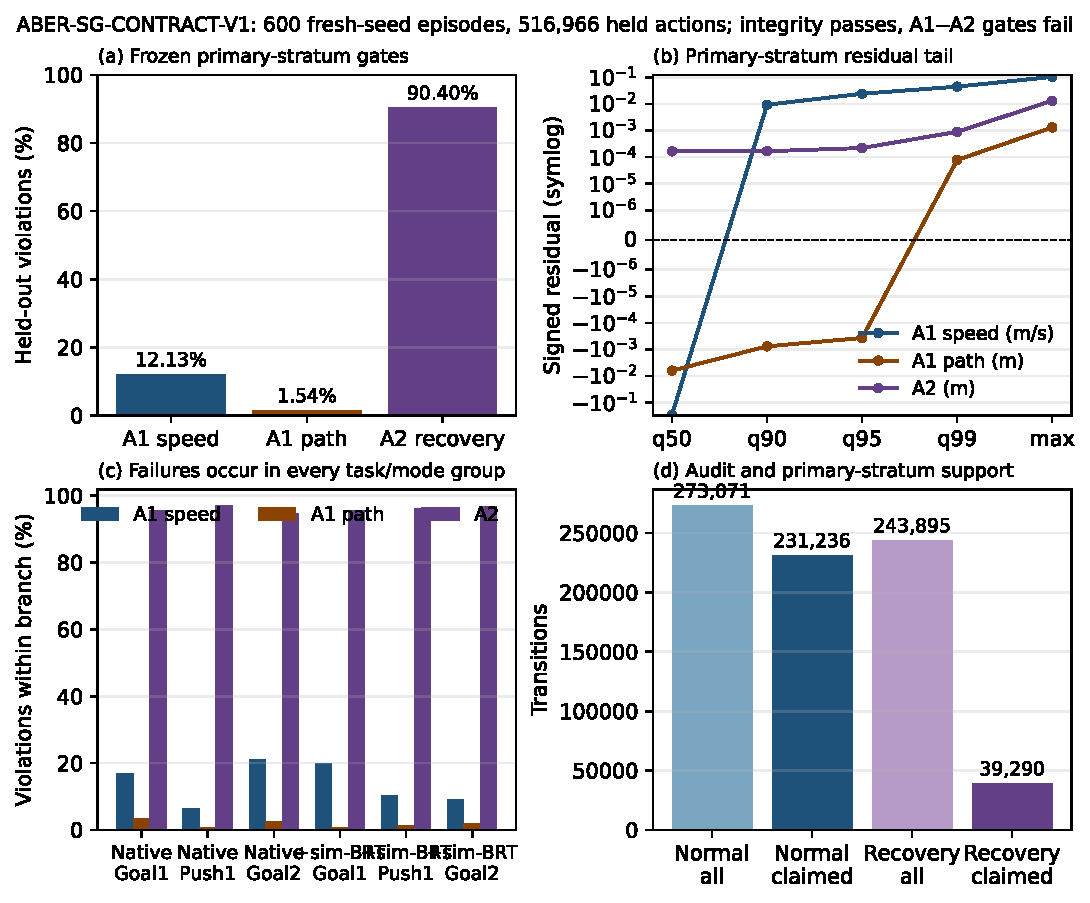
\includegraphics[width=\linewidth]{../figures/supplement/aber_safetygym_contract_v1.pdf}
\caption{The held-out contract audit.  Failures remain after excluding every
hold with non-ground contact and occur in every task/training-mode group.}
\label{fig:sg-contract-v1}
\end{figure}

The V1 decision is therefore a \emph{no-go} for connecting the current
$a_b=0.9$, $v_{\max}=1.5$, $\Delta t=0.02$ Safety-Gym experiments to the
unmodified A1--A2 envelope.  This is not a failure of the conditional theorem
or a retraction of the paired empirical collision comparison.  It establishes
the sharper boundary: the model-matched benchmark tests the theorem under its
assumptions, whereas the Safety-Gym matrix remains empirical and cannot be
called theorem validation.  In particular, current Safety-Gym data do not
certify $(0,0)$ as the required recovery and do not yet justify MuJoCo
ABER-FP directional-tube confirmation.

The complete frozen protocol, aggregate audit, raw gzip traces, collector,
substep instrumentation, independent auditor, plotting script, and focused
tests are included in the reproducibility materials.  A successor contract
must be separately named and pre-frozen.  It may restrict the accepted
operating region or use a conservative measured envelope conditioned on
starting speed, executed forward/turn commands, actuator mode, and contact
topology; it must not reinterpret V1 or tune a constant to these held-out
failures.


\section{Conditional Directional Fast Path}

\paragraph{Why the intervention rule must change.}
The original ABER cap is maximal under the bearing-independent A1 envelope
proved in the main paper.  Raising that cap by threshold tuning would discard
the premise that makes the cap safe.  We therefore study ABER-FP, a
conditional extension that credits a favorable turn only when a stronger
executed-transition certificate is available, and otherwise returns the
unchanged ABER action.

\paragraph{Directional transition contract.}
For candidate action $u$, let $\Gamma(x,u)$ be a sound tube containing the
complete realized position trace over the next hold interval, let
$\bar s^+(x,u)$ upper-bound the next translational speed, and let
$\underline d_i^+(x,u)$ lower-bound endpoint clearance to obstacle $i$.
ABER-FP accepts $u$ only if
\begin{align}
 \min_{y\in\Gamma(x,u)}\|y-o_i\|-r_i &\ge 0,
 \label{eq:fppath}\\
 \underline d_i^+(x,u)-D(\bar s^+(x,u)) &\ge 0
 \quad\text{for every }i.
 \label{eq:fpend}
\end{align}
Equation~(\ref{eq:fppath}) prevents intersample keepout entry, while
(\ref{eq:fpend}) returns the next sample to the original ABER set
$\mathcal C$.

\paragraph{Complete online algorithm.}
Let $u_{\rm RL}=(f,w)$ after range clipping and first compute
$u_{\rm base}=\operatorname{ABER}(x,u_{\rm RL})$.  Form
\[
 F=f\{1,.75,.5,.25,0\},
\]
\[
 W=\operatorname{unique}\{\operatorname{clip}(w),\
 \operatorname{clip}(w-.5),\
 \operatorname{clip}(w+.5),-1,0,1\}.
\]
The candidate library is
$Q=\operatorname{unique}((F\times W)\cup\{u_{\rm base}\})$, hence
$|Q|\le31$.  Sort $Q$ by increasing
$\|u-u_{\rm RL}\|_2^2$.  Return the first candidate satisfying
(\ref{eq:fppath})--(\ref{eq:fpend}) for every obstacle; if none passes,
return $u_{\rm base}$.  For $m$ obstacles and the fixed library size, the
online work is $O(31m)=O(m)$ and uses no optimization, fitting, interpolation,
or actor update.

\paragraph{Safety composition.}
\textbf{Proposition S1.}  Suppose the original ABER assumptions A1--A2 hold
and the directional contract is sound for every accepted fast-path action.
Starting in $\mathcal C$, ABER-FP has the same sampled and intersample safety
conclusion as ABER.

\emph{Proof.}
If a fast-path candidate is accepted, (\ref{eq:fppath}) keeps its complete
held trace outside every keepout and (\ref{eq:fpend}) places its endpoint in
$\mathcal C$.  If no candidate is accepted, the output is exactly
$u_{\rm base}$, for which the original ABER theorem preserves the same two
properties.  Induction over sample intervals proves the claim. \hfill$\Box$

The proposition is a composition result, not a finite-data guarantee for a
learned tube.  In the deterministic differential-drive benchmark,
$\Gamma(x,u)$ is the exact held line segment and the endpoint is the exact
semi-implicit servo transition, so the premise is exact.  Safety-Gym and
hardware deployment require a separately frozen, held-out accepted path tube;
the current 20 braking traces do not validate this directional premise.
Accordingly, ABER-FP is not enabled in the MuJoCo claims of the main paper.

\begin{table*}[t]
\centering
\small
\setlength{\tabcolsep}{5pt}
\begin{tabular}{llrrrrr}
\toprule
Scene & Method & Collision & Success & Intervention & Recovery/episode
& Success time (s)\\
 & & (\%) & (\%) & step fraction (\%) & & \\
\midrule
Single & ABER    & 0 & 100 & 49.73 & 8.57  & 6.440\\
Single & ABER-FP & 0 & 100 & 23.33 & 0     & 5.265\\
Multi  & ABER    & 0 & 100 & 83.01 & 13.61 & 7.308\\
Multi  & ABER-FP & 0 & 100 & 34.49 & 0     & 6.286\\
\bottomrule
\end{tabular}
\caption{Frozen held-out comparison in the exact differential-drive model.
Each method/scene cell uses 500 non-development seeds.  All 2,000 runs have
zero certificate violations.}
\label{tab:fastpathheldout}
\end{table*}

\begin{figure*}[t]
\centering
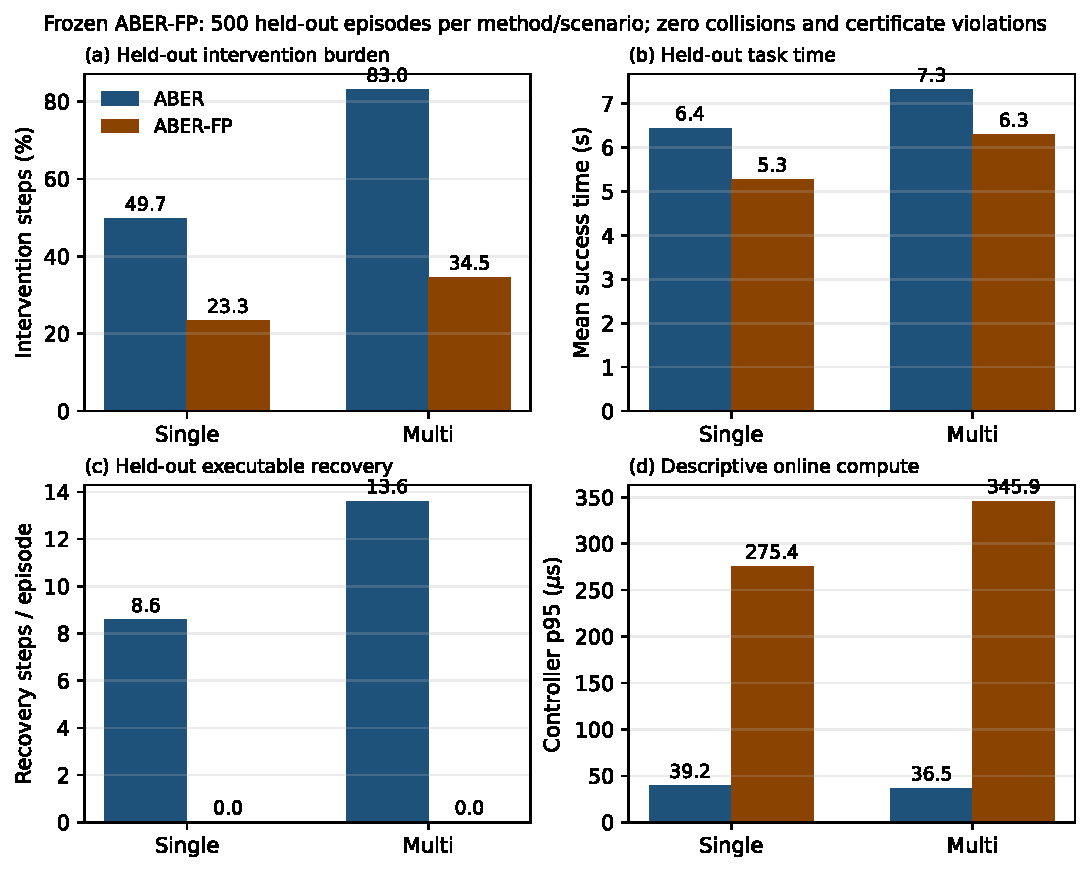
\includegraphics[width=\textwidth]{../figures/supplement/aber_fastpath_performance.pdf}
\caption{Held-out task and intervention performance, with descriptive
controller latency.  ABER-FP lowers intervention occupancy by 53.08\% in the
single-obstacle scene and 58.45\% in the multi-obstacle scene, while reducing
mean success time by 18.24\% and 13.98\%, respectively.}
\label{fig:fastpath}
\end{figure*}

The added check raises controller p95 latency from 39.2 to 275.4~$\mu$s in the
single-obstacle scene and from 36.5 to 345.9~$\mu$s in the multi-obstacle
scene.  The latter is 1.73\% of a 20-ms control period.  These wall times are
machine-specific descriptive measurements; the fixed-library $O(m)$ bound
follows from the implementation.

The executable implementation is
\path{experiments/aaai/aber_fastpath_benchmark.py}; tests are in
\path{tests/test_aber_fastpath.py}.  Frozen development, held-out, and runtime
records are respectively \path{data/aber_fastpath_benchmark.json},
\path{data/aber_fastpath_heldout.json}, and
\path{data/aber_fastpath_runtime.json}.


\section{Reproduction and Data Boundary}

The local evidence bundle contains a checksum manifest, all 30 evaluation
summaries and resolved configurations, all 30 checkpoints, runtime and paired
raw records, and a one-command verifier:
\begin{quote}
\path{./verify_artifact.sh}
\end{quote}
Its individual commands are:
\begin{quote}
\noindent\path{PYTHONPATH=.}\ \path{pytest}\ \path{-q}\ \path{tests/test_brake_manifold_sampled_data.py}\par
\noindent\path{PYTHONPATH=.}\ \path{pytest}\ \path{-q}\ \path{tests/test_aber_fastpath.py}\par
\noindent\path{PYTHONPATH=.}\ \path{pytest}\ \path{-q}\ \path{tests/test_aber_component_ablation.py}\par
\noindent\path{PYTHONPATH=.}\ \path{pytest}\ \path{-q}\ \path{tests/test_aber_contract_trace.py}\par
\noindent\path{PYTHONPATH=.}\ \path{python}\ \path{experiments/aaai/audit_aber_safetygym_contract_v1.py}\par
\noindent\path{PYTHONPATH=.}\ \path{python}\ \path{experiments/aaai/certify_aber_properties.py}\par
\noindent\path{PYTHONPATH=.}\ \path{python}\ \path{experiments/aaai/certified_diffdrive_benchmark.py}\par
\noindent\path{PYTHONPATH=.}\ \path{python}\ \path{experiments/aaai/aber_fastpath_benchmark.py}\par
\noindent\path{PYTHONPATH=.}\ \path{python}\ \path{experiments/aaai/aber_fastpath_heldout.py}\par
\noindent\path{PYTHONPATH=.}\ \path{python}\ \path{experiments/aaai/aber_fastpath_runtime.py}\par
\noindent\path{PYTHONPATH=.}\ \path{python}\ \path{experiments/aaai/aber_component_ablation.py}\par
\noindent\path{PYTHONPATH=.}\ \path{python}\ \path{experiments/aaai/aggregate_aber_matrix.py}\par
\noindent\path{PYTHONPATH=.}\ \path{python}\ \path{experiments/aaai/aggregate_aber_paired_matrix.py}\par
\noindent\path{PYTHONPATH=.}\ \path{python}\ \path{experiments/aaai/analyze_aber_interventions.py}\par
\noindent\path{PYTHONPATH=.}\ \path{python}\ \path{experiments/aaai/verify_aber_paired_matrix.py}\par
\noindent\path{PYTHONPATH=.}\ \path{python}\ \path{experiments/aaai/audit_aber_latched_restore_cross_task_multiseed.py}\par
\noindent\path{PYTHONPATH=.}\ \path{python}\ \path{experiments/aaai/aggregate_aber_latched_restore_full_matrix.py}\par
\noindent\path{PYTHONPATH=.}\ \path{python}\ \path{experiments/aaai/verify_aber_extended_evidence.py}
\end{quote}
The matrix-aggregation command validates existing raw run directories before
rewriting the JSON aggregate and main-paper table.  It does not synthesize
missing cells.  If any raw run or saved configuration is absent, it fails
rather than imputing a value.

The property, reference, component, and runtime artifacts record
Python~3.13.9 and NumPy~2.4.6.  The paired rollout used Python~3.10.19,
NumPy~1.23.5, PyTorch~2.10.0, and Safety-Gymnasium~1.2.0.  The anonymous
artifact regenerates the deterministic benchmarks, validates all 30
checkpoint and raw-rollout hashes, and recomputes the full-matrix statistics
from frozen audit outputs.  Full policy retraining requires the larger
external training environment and is outside the minimal artifact.
Diagnostic files unrelated to the method and claims in this paper are
excluded from the anonymous evidence package.

\end{document}
